\chapter{Introduction}
\label{ch:Introduction}
Conventional energy resources such as fossil fuels and nuclear energy are not only limited but also pose adverse effects on the environment. Therefore, we are striving to find a cheap and renewable source of energy. Wind energy is such source of energy and is getting more popular, and have also become more affordable. Novel renewable technologies such as \indexAcron{Vertical-Axis Wind Turbine}{VAWT} are now a promising research field that can satisfy this growing demand.

	\begin{figure}[!b]
        \centering
        \begin{subfigure}[b]{0.25\textwidth}
                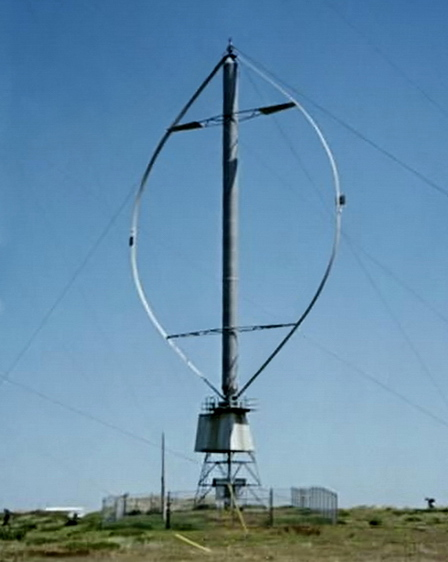
\includegraphics[height=0.2\textheight]{figures/introduction/Darrieus-windmill.jpg}
                \caption{VAWT: Darrieus wind turbine\cite{darrieusWindmill}}
                \label{fig:Darrieus-windmill}
        \end{subfigure}%
        \qquad \qquad%add desired spacing between images, e. g. ~, \quad, \qquad etc.
          %(or a blank line to force the subfigure onto a new line)
        \begin{subfigure}[b]{0.25\textwidth}
                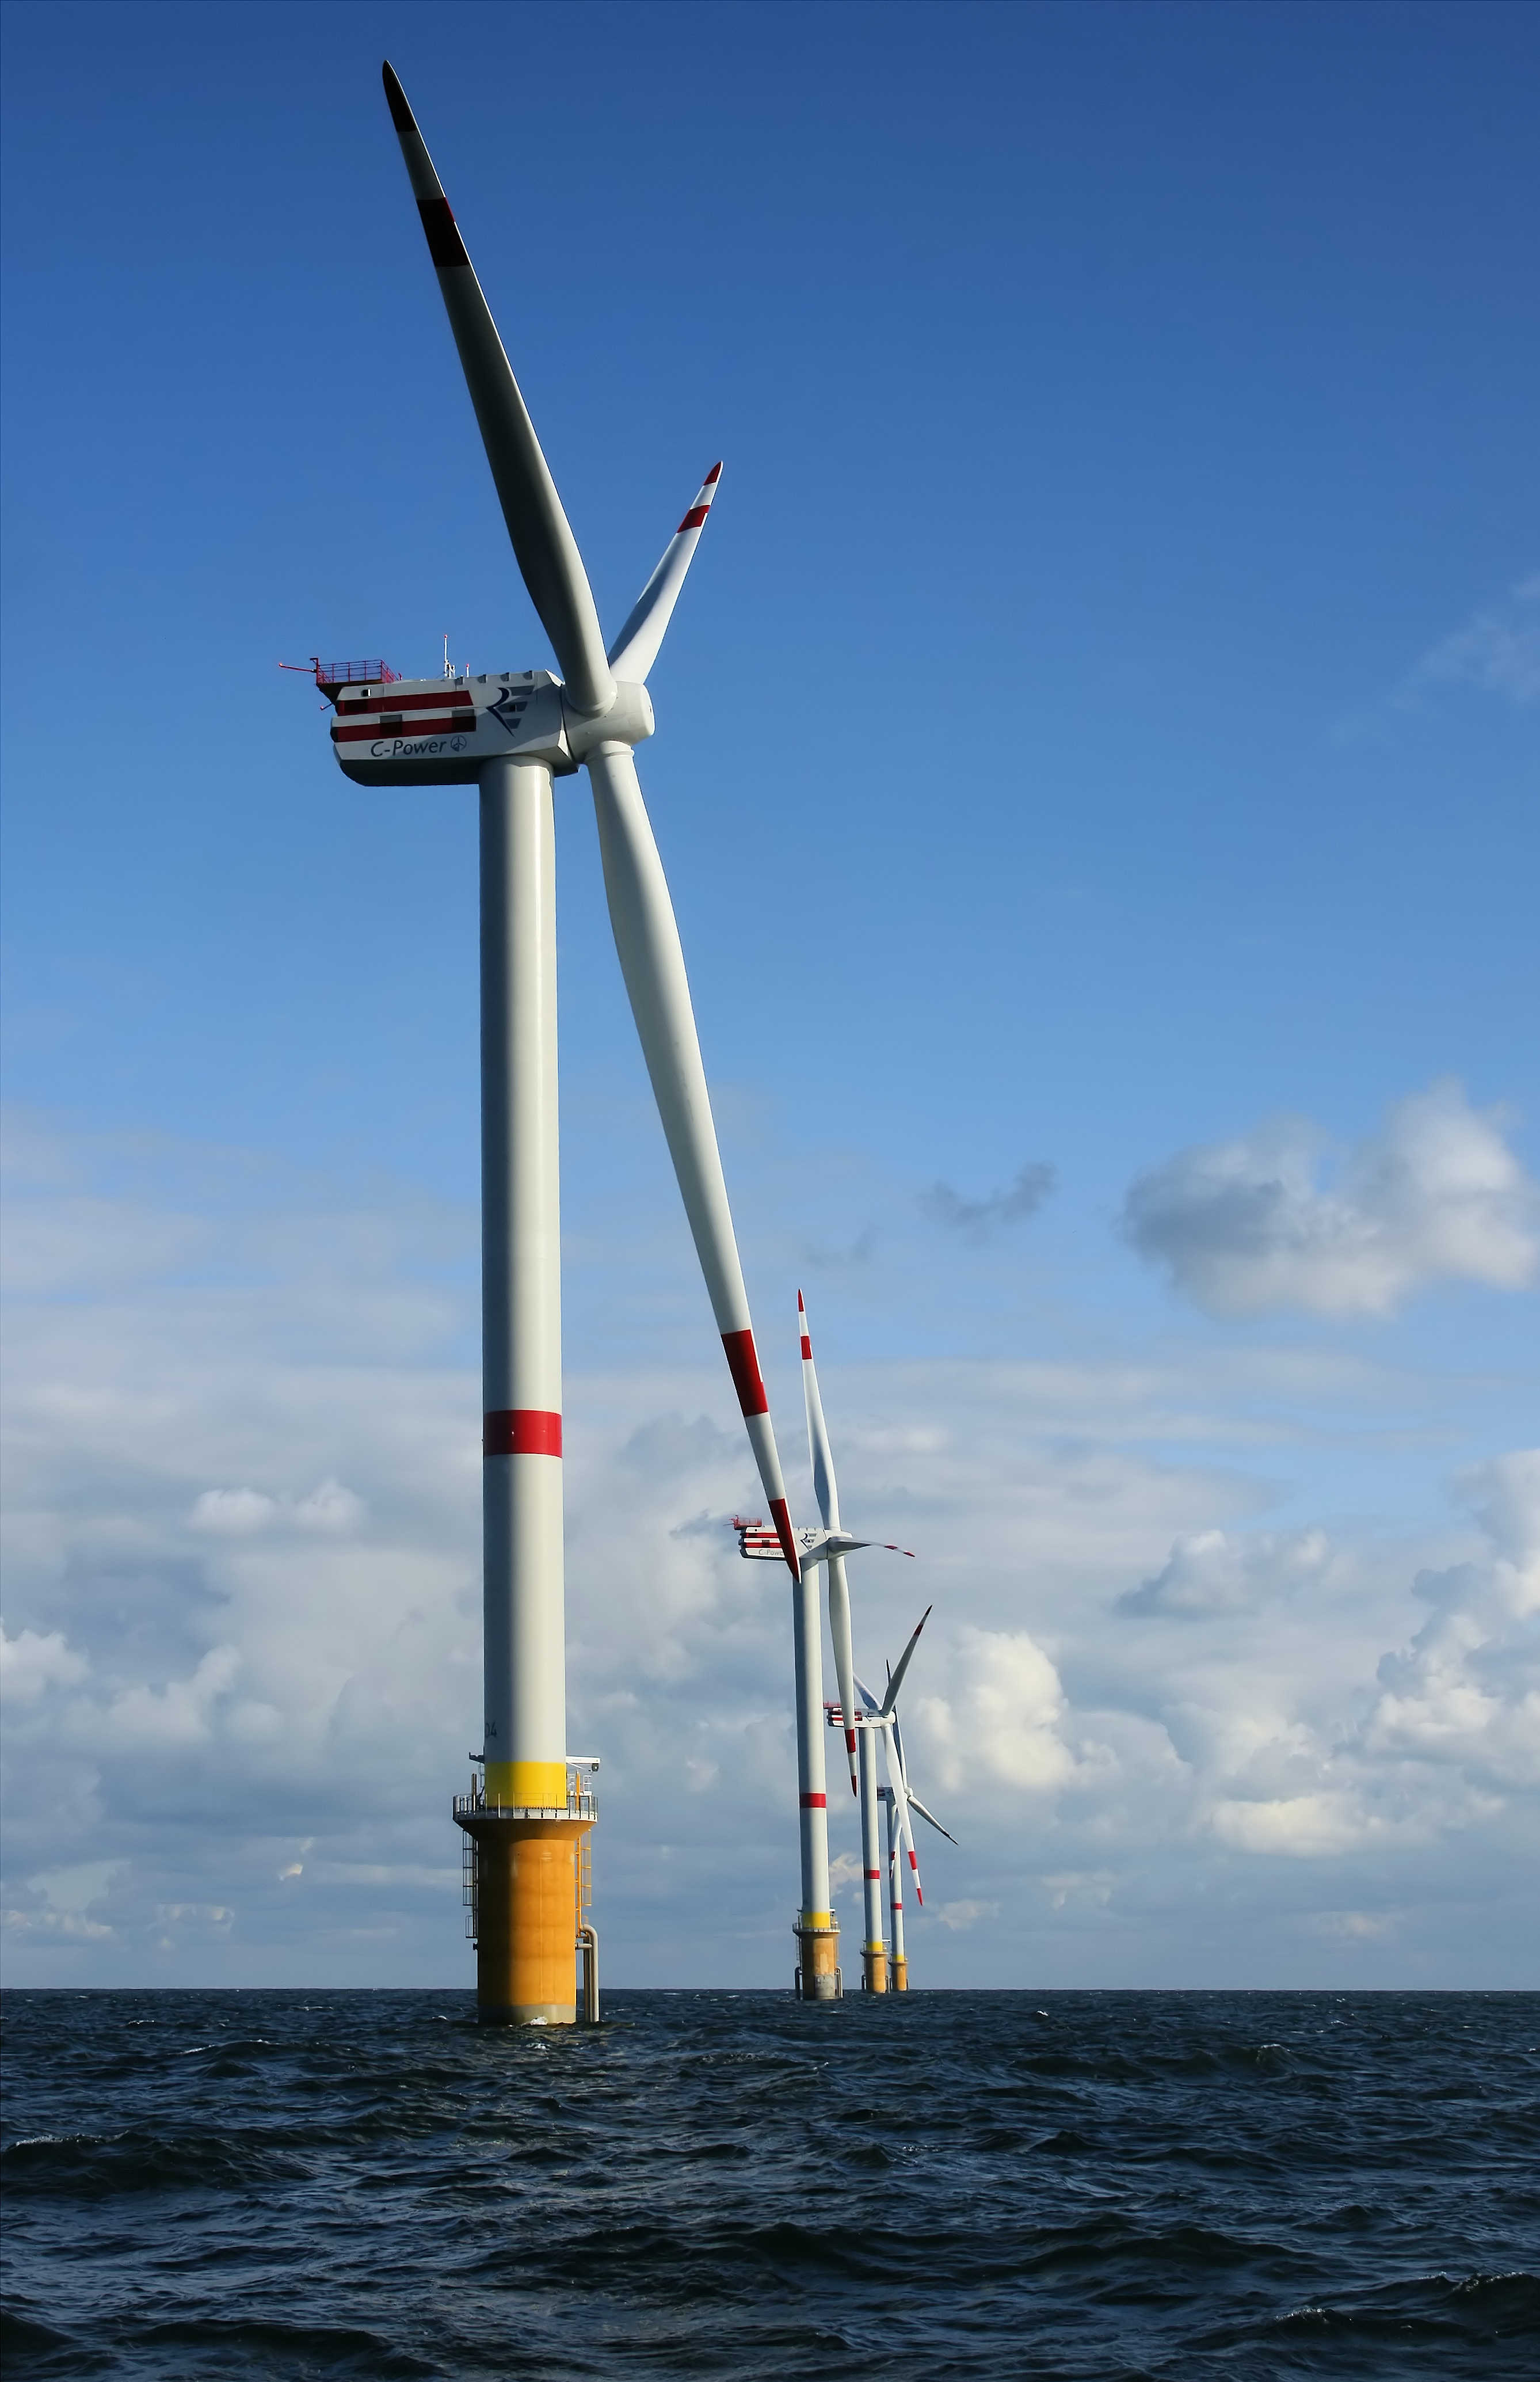
\includegraphics[height=0.2\textheight]{figures/introduction/HAWT_compressed.jpg}
                \caption{HAWT: Offshore wind turbine \cite{HAWTWindmill}}
                \label{fig:HAWT}
        \end{subfigure}
        \caption{VAWT vs. HAWT}
        \label{fig:VAWTvsHAWT}
	\end{figure}

VAWT are unlike the normal wind turbine, which are mounted on a mast away from the ground and generates energy by spinning perpendicular to the ground, figure \ref{fig:VAWTvsHAWT}. Whereas the VAWT, figure \ref{fig:Darrieus-windmill}, spins parallel to the ground with its hub located at the ground \cite{website:wikiVAWT}. The advantages of the VAWTs are what makes them ideal for a source of renewable energy. As the turbine is located at the ground, it is easily accessible and is easily maintained. The second main advantage of the VAWT is the way it dissipates its wake. Near-wake experiments of Ferreira (2009) \cite{Ferreira}, and simulations of Vermeer (2003) \cite{Vermeer2003} have shown that the fluid past the turbine is more turbulent. Due to this higher mixing, the flow is able to recover much earlier than the convectional wind turbines. This means that it possible to places VAWTs much closer to each other and so a VAWT farm can potentially give more power per area. Furthermore, VAWTs operate independent of the flow direction, and can operate at low wind speeds (i.e. at low tip-speed ratios).

However, there are some limitations that we must take into account. As the blades passes through its own wake, complex wake-body interactions take places, figure \ref{fig:3DunsteadyPanelVAWT}. These have adverse effect on the blade structure, making it more susceptible to fatigue. As the blade is constantly pitching, flow behaviors such as dynamic stall and constant vortex shedding takes place \cite{SimaoFerreira2008}. This complex fluid behaviors makes it hard to predict the performance of a VAWTs and this is one of the reasons why VAWTs are not widely used. 

	\begin{figure}[!t]
		\centering
		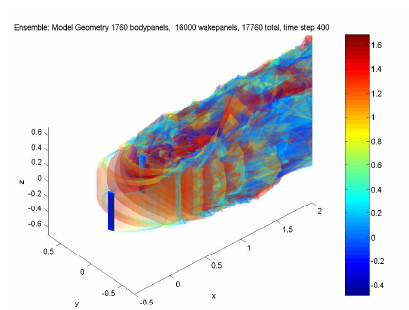
\includegraphics[width=0.6\linewidth]{figures/introduction/3DunsteadyPanelVAWT.png}
		\caption{3D Unsteady Panel simulation of a Straight-bladed VAWT showing the strength of the shed vorticity. The VAWT blades interact with its own wake increasing the complexity of the wake geometry \cite{Dixon}}
		\label{fig:3DunsteadyPanelVAWT}
	\end{figure}

In addition, the VAWT operates at large Reynolds number making accurate numerical methods computationally very expensive. So we see that we require a numerical method that is not reproduce accurate results, but is also efficient at modeling the flow around the turbine.

\section{Motivation and Goal}
The goal of the research is to develop an efficient, reliable, and accurate numerical method for modeling the flow around a \indexAcron{Two-Dimensional}{2D} VAWT, enabling to deduce its correct performance characteristics. The two approaches of investigating the flow around a turbine is by either using a numerical method to model the flow, or by performing a real-life experimental tests, such as a wind tunnel experiment.

To understand the unsteady aerodynamic behavior, \indexAcron{Particle Image Velocimetry}{PIV} has been a useful tool to visualize the flow around the turbine. PIV was used by Ferreira et al. (2007) \cite{Ferreira2007}, have shown that it was possible to acquire flow characteristics around the blade, and the simulations have been useful at validating the numerical methods for the VAWT. The downside to experimental investigation is that is it very expensive to investigate all types of airfoil geometries, blade geometries and VAWT configurations. However, investigation this is vital in understanding the performance characteristics of VAWT. Furthermore, the model sizes are limited by the dimensions of the wind tunnel, and investigations with arrays of VAWTs in a wind tunnel is difficult.

Numerical methods are therefore a popular alternative as the cost of simulation is becoming progressively smaller, and the accuracy of the models are increasing day by day. In the research field, there exists many models with various orders of accuracy. \indexAcron{Actuator Disk}{AD} and \indexAcron{Blade Element Momentum}{BEM} models are the simplest models, built upon satisfying the momentum balance of the turbine with the fluid. The advantage is that they are very quick, however they lack the accuracy that are obtained by experimental simulation. Complex blade-wake interactions such as dynamic stalls and flow separations cannot be modeled by these methods, and therefore we must rely on more powerful tools.

	\begin{figure}[!t]
		\centering
		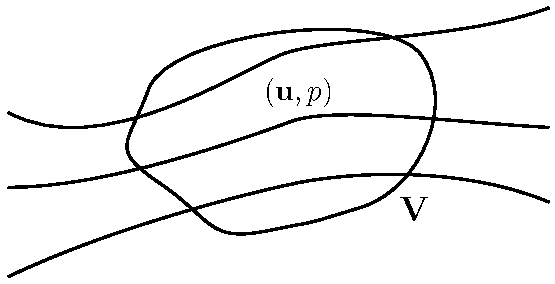
\includegraphics[width=0.4\linewidth]{figures/introduction/eulerianRF.pdf}
		\caption{Eulerian formulation of the fluid. We observe a given volume $\mathbf{V}$ and evaluate the change in properties of the fluid (from incompressible flow: velocity $\mathbf{u}$ and pressure $p$) at time passes.}
		\label{fig:eulerianRF}
	\end{figure}

To ensure more accuracy, one has to solve the Navier-Stokes equation of the flow around the turbine without large simplifications. \indexAcron{Computional Fluid Dynamic}{CFD} methods discretizes the fluid into smaller regions and solves the Navier-Stokes equation in each region (or grids). This type of formulation is known as an Eulerian formulation as we are evaluating the change in flow property of a given region, figure \ref{fig:eulerianRF}. In order to fully resolve the flow around the turbine, we would have to discretize the fluid very small at the blade where the vortex cores are very small, and we would need large grids far away from the blades where the vortex cores are much larger. Therefore, we would need grid size of various order of magnitudes at various regions of the fluid. This requires a large number of grids, and furthermore as the blades are constantly moving, this introduction additional limitations when defining the problem in Eulerian formulation.

An alternative method is to use the vortex formulation of the Navier-Stokes equations, referred to as vorticity equation. This method is ideal because when describing it in Lagrangian formulation, the evolution of the vorticity is resulted from the interaction between vortices in the fluid. The removes the requirement of grids, figure \ref{fig:lagrangianRF}. In addition, using simulation acceleration methods such as \indexAcron{Fast Multipole Method}{FMM} and parallel computation in \indexAcron{Graphical Processing Units}{GPU}, they are much more efficient that typical CFD methods. However, vortex method cannot inherently take in account the solid body. They require additional methods that can describe the effect of the body in the fluid and the vorticity generated from the body.

	\begin{figure}[!t]
		\centering
		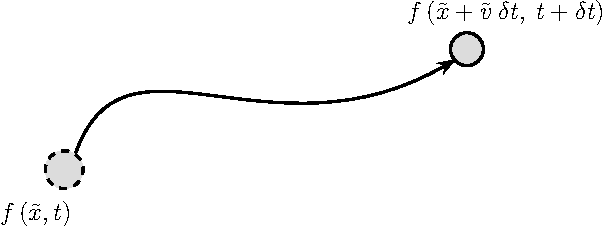
\includegraphics[width=0.4\linewidth]{figures/introduction/lagrangianRF2-crop.pdf}
		\caption{Lagrangian formulation of the fluid. We track the path of the individual fluid elements as time passes.}
		\label{fig:lagrangianRF}
	\end{figure}

So, we see that Eulerian method is accurate when describing the blade-wake interaction but not efficient when describing multi-scale domains. The Lagrangian method is very efficient in evolving the vorticity of the fluid. Due to auto-adaptive nature of the Lagrangian method, it is an ideal choice when describing the multi-scale flow characteristics. However, it is not efficient in resolving the near-body region, where the vorticity is generated. Therefore, in order to use the advantage of both methods, we have decided to use a domain-decomposition method, referred to as \indexAcron{Hybrid Eulerian-Lagrangian Vortex Particle Method}{HELVPM}. In this method, the Eulerian grid method will be used at the region around the blade (i.e. the near-wall region). The Lagrangian vortex method will be used in the wake region of the body. With proper coupling of these methods, we can ensure that this numerical method can capture not only the near-wake phenomenons such as vortex shedding, dynamic stall, and the wake-body interaction, but also the large-scale flow structures such as the evolution of the VAWT wake.

\section{Research Aim and Plan}

We have formulated research that can help us accomplish our goal. The research question that are derived from the gaol of the project is as follows:

\paragraph*{Research Questions:}
	\begin{itemize}
	\item \textit{Is it possible to develop an efficient and accurate numerical method by an
	hybrid approach, with the vortex particle method solving the wake, and the Navier-Stokes grid solver solving the near-body region?}
	
	\item \textit{Will it be able to predict similar performance characteristics and flow phenomena as observed from the wind tunnel experimental setup?}
	
	\item \textit{Will it be capable of simulating the blade-wake interaction and the dynamic stall?}
	
	\item \textit{Where are the errors and what are their sources?}
	\end{itemize}
%\textit{Is it possible to develop an efficient and accurate numerical method by an
%hybrid approach; where the vortex particle method is used in the wake, and the Navier-Stokes grid solver is
%used at the near-body region? Will it be able to simulate real life performance characteristics of a Vertical-Axis Wind Turbine? Will it be able to predict similar performance characteristics and flow phenomena as observed from the wind tunnel experimental setup? Will it be capable of simulating the blade-wake interaction
%and the dynamic stall? Where are the errors and what are their sources?}

In order to answer the research questions, the goal of the project is the develop an efficient and accurate
numerical method that is not only capable of capture the small scale flow phenomena such as the dynamic stall and the vortex shedding, but is also efficient at modeling the evolution of the wake. The investigation will be performed for 2-D geometries and the accuracy of the model needs to established first for simple problems before investigating more we can tackle complicated problems. In other words, the initial goal is to develop the hybrid vortex particle method and verify the approach. During this process, the solver will be verified and validated against test cases starting from simpler problems and gradually developing more complex features.

The investigation is currently possible for 2-D simulations because full 3-D simulations are beyond the scope of the thesis. This is mainly due to the lack of research period that we have at hand. However, 3-D simulation can simply be extended from the accomplishments of the 2-D development work. A final goal would have been to investigate the VAWT performance, however due to time constrictions, it too was beyond the scope of the thesis. Thus we can now summarize the aim and the plan of the research.

\paragraph*{Research aim and plan:}
\textit{
	\begin{itemize}
	\item Develop the Hybrid method for capturing small-scale phenomenons and large scale phenomenons.
	\item Ensure this tool is efficient, reliable, and accurate.
	\item Verify and validate the tools with test cases.
	\end{itemize}
}
The innovativeness of this project is that such hybrid modeling has not been yet applied for the wind energy problem case. Through the parallelization of the vortex particle method in a GPU and employing solver acceleration techniques such as the FMM, this simulation could give an edge in the understanding the flow behavior of a VAWT.

\section{Introduction to Hybrid Eulerian-Lagrangian Vortex Particle Method}

The \indexAcron{Hybrid Eulerian-Lagrangian Vortex Particle Method}{HVM} is a domain-decomposition method, where the Eulerian method and the Lagrangian method solves different domains of the fluid. The domain decomposition method is simply splitting the domain of interest and using the appropriate methods in each domain. For the problem of VAWT, as the boundary is non-trivial and is the source of vorticity, the full Navier-Stokes model will be used here, and away from the body where only the convection of the vorticity field is interested, the fast and efficient vortex particle method will be used, figure \ref{fig:domainDecomposition}.

Several researches have already been done: Cottet and Koumoutsakos (2000a)\cite{Cottet2000a}, Guermond and Lu (2000) \cite{Guermond2000} simulated the advection dominated flows; Ould-Salhi et al. (2001) \cite{Ould-Salihi2001} blended the finite difference and vortex method together; Winckelmans et al. (2005a) \cite{Winckelmans2005a} investigated the trailing vorticies; Daeninck (2006) \cite{Daeninck2006} used a simplified coupling strategy, coupling Vortex Particle Method and Finite Diference Method; Stock (2010) \cite{Stock} expanded Daeninck's strategy, coupling Vortex Particle Method and Finite Volume Method and modeled a 3-D rotor.

When evaluating the previous works, we see that not all domain decomposition methods are the same. The main difference difference between the methods is their coupling strategies. Most works employ the Schwartz alternating method to couple the vortex particle method and the grid solver. The Schwartz alternating method (or sometimes referred to as Schwartz iterative method), couples the vortex particle method and the grid solver by iteratively determining the boundary condition such that the stream functions in both domains, $\psi_L$ and $\psi_E$ in $\Omega_L$ and $\Omega_E$ respectively, match at the overlap region $\Omega_E-\Omega_L$. Figure \ref{fig:domainDecomposition} shows the domain decomposition using the Schwartz alternating method. The summary of a single iteration of the Schwartz alternating method is as follows:
	\begin{itemize}
	\item Determine the Eulerian boundary condition, the stream function $\psi_{\Gamma_E}$ at the Eulerian boundary $\Gamma_E$, extracted from the Lagrangian stream function $\psi_L$in the Lagrangian domain $\Omega_L$.
	\item Solve for the stream function $\psi_E$ in the Eulerian domain $\Omega_E$ with the new boundary condition $\Gamma_E$.
	\item Determine the Lagrangian condition, the stream function $\psi_{\Gamma_L}$ at the Lagrangian boundary $\Gamma_L$, extracted from the Eulerian stream function $\psi_E$ in the Eulerian domain $\Omega_E$.
	\item Solve the stream function $\psi_L$ in the Lagrangian domain with the boundary conditions $\psi_{\Gamma_L}$ at the Lagrangian boundary $\Gamma_L$.
	\end{itemize}
	
This procedure is iterated until the stream functions of both the domains converges \cite{Ould-Salihi2001}. Onces the stream function is determined in both the domains, the velocity field can be obtained. Using the velocity field, we can evolve the vorticity field in both the domain. 

As we realized now, the downside to this procedure is that we have solve the stream functions in both $\Omega_E$ and $\Omega_L$ iteratively, till we converge to a solution. This makes the computation very expensive, especially when we are dealing with large number of vortex particles. Therefore, for this project, we are using the coupling techniques that is based on the research work of Daeninck (2006) \cite{Daeninck2006} and Stock (2010) \cite{Stock}.

	\begin{figure}[!t]
		\centering
		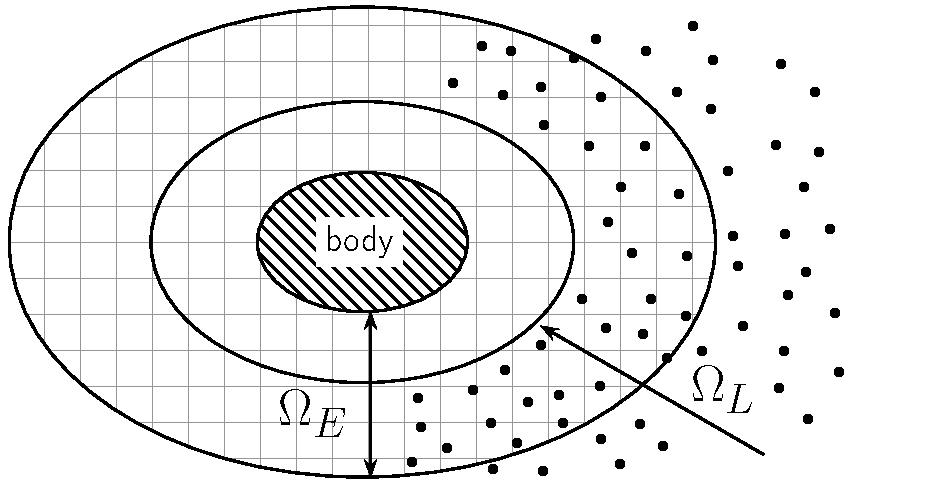
\includegraphics[width=0.6\linewidth]{figures/introduction/domainDecomposition_typical_type2.pdf}
		\caption{Standard domain decomposition using Schwartz iteration for coupling the two methods. Eulerian domain $\Omega_E$ (near the body), and Lagrangian domain $\Omega_L$ (away from the body). Figure is based on Guermond (2000) \cite{Guermond2000}}.
		\label{fig:domainDecomposition}
	\end{figure}

\subsection{Simple coupling strategy}
This approach will be referred to as the \indexAcron{Simple Coupling Strategy}{SCS}. It is simpler that the Schwartz iterative method, as no iteration is needed for the coupling procedure. The basic procedure is to solve the vortex method in the full fluid domain using relatively coarse resolution of the near-wall region. Then we use the grid solver in the near-wall region to capture the detailed features of the boundary layer and transfer the vorticity field at this region to the vortex particles, figure \ref{fig:domainDecomposition_daenick}. Therefore, the grid solver basically acts as the correction for the under-resolved regions of the Lagrangian method. The functionality of this strategy has been demonstrated by Daeninck and was found to be significantly faster than the Schwartz coupling strategy. The features of the simple coupling strategy can summarized as follows:

	\begin{itemize}
	\item Eulerian method is used to resolve the near-wall region, at the Eulerian domain $\Omega_E$, enabling it to capture important features of the boundary layer (such as flow separation) with great accuracy.
	
	\item Lagrangian method is used to capture the wake, at the Lagrangian domain $\Omega_L$, and to efficiently evolving the wake.
	
	\item The accurate solution of the Eulerian domain is transfered to the Lagrangian domain according to the coupling algorithm of Daeninck \cite{Daeninck2006} and Stock \cite{Stock}.
	
	\item The boundary conditions for the Eulerian domain is retrieved from the Lagrangian domain.
	\end{itemize}

	\begin{figure}[!t]
		\centering
		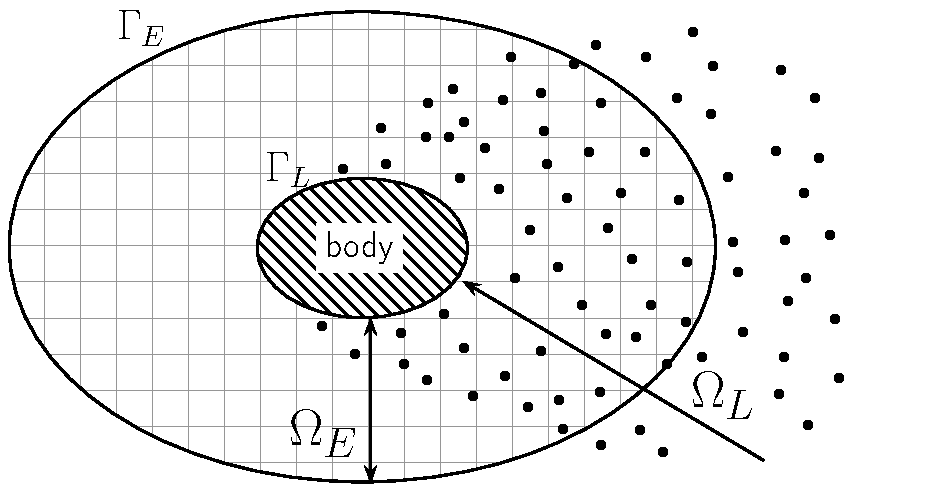
\includegraphics[width=0.6\linewidth]{figures/introduction/domainDecomposition_daenick_type2.pdf}
		\caption{Modified domain decomposition \underline{without} Schwartz alternating method. Lagrangian domain extends up to the surface of the body. Figure is based on Daeninck (2006) \cite{Daeninck2006}.}
		\label{fig:domainDecomposition_daenick}
	\end{figure}

The algorithm to the \printAcron{Simple Coupling Strategy}{SCS} follows from Daeninck's doctoral thesis, \cite{Daeninck2006}. Figure \ref{fig:flowchart_simpleCoupling} shows the overview to the algorithm and can be summarized as follows:

	\begin{enumerate}
	\item \textbf{Correct Lagrangian:} Use the solution of the Eulerian domain $\Omega_E$ (in the near-wall region) to correct the solution of the Lagrangian domain $\Omega_L$, that is overlapping the Eulerian domain.  
	
	\item \textbf{Evolve Lagrangian:} With the modified solution, evolve the Lagrangian solution from time step $t_n$ to next time step $t_{n+1}$.
	
	\item \textbf{Determine Eulerian boundary conditions:} Use the Lagrangian solution of time $t_n$ and $t_{n+1}$ to determine the boundary conditions of the Eulerian domain.
	
	\item \textbf{Evolve Eulerian:} With the boundary condition, evolve the Eulerian solution from $t_n$ to $t_{n+1}$.
	\end{enumerate}
	
This is the basic approach for coupling the Eulerian method in the Eulerian domain $\Omega_E$ with the Lagrangian method in the Lagrangian domain $\Omega_L$ without the iterative Schwartz algorithm. 

Furthermore, the SCS handles the Lagrangian boundary condition differently from the classic hybrid method. Typically during the evolution process of the Lagrangian domain, the shedding of the vorticity is also defined in the Lagrangian method. However, in our coupling strategy, the Lagrangian method is under-resolved at the boundary and cannot be used to resolve the vorticity flux at the body. Instead, we use the Eulerian method to resolve the boundary, and the Eulerian method acts as the vorticity generator for the Lagrangian method. However, there as some assumptions that we must satisfy, for this coupling strategy to be valid:

	\begin{itemize}
	\item At $t_n$, before the evolution of both method to $t_{n+1}$, the Lagrangian solution matches Eulerian solution at the near-wall region.
	\item After the evolution to $t_{n+1}$, the deviation of the Lagrangian solution (due to lack of vorticity flux at Lagrangian boundary), should be minimal.
	\item Even though the Lagrangian domain is under-resolved in the near-wall region, it should be able to provide accurate boundary conditions for the Eulerian external boundary.
	\end{itemize}
	
	\begin{figure}[!t]
		\centering
		\begin{tikzpicture}
			[node distance=.8cm, start chain=going below,]
			\node[punktchain, join] (correct) {Correct the Lagrangian domain};
		    \node[punktchain, join] (evolveL) {Evolve the Lagrangian solution};
		    \node[punktchain, join] (bcE)     {Determine the Eulerian boundary conditions};
		    \node[punktchain, join] (evolveE) {Evolve the Eulerian solution};
		\end{tikzpicture}
		\caption{Flowchart of the simple coupling strategy. The flowchart shows the procedure to evolve both methods from $t_n$ to $t_{n+1}$.}
		\label{fig:flowchart_simpleCoupling}
	\end{figure}

\section{Verification and Validation Test Cases}

The test-cases that are used for this thesis are summarized as given:

	\begin{description}
	\item[Lamb-Oseen vortex] \cite{Lamb1993} \cite{Tryggeson2007} \hfill\\
	Lamb-Oseen vortex test case is an analytical solution derived from the diffusion equation, and is a test case for unbounded flow (without any wall). This is the first model that will be used to validate the Lagrangian method and Eulerian method separately. This test case focuses on the evolution of the vorticity field and therefore is an ideal test case to verify and validate the convection and diffusion of the vorticity.
	\item[Clercx-Bruneau dipole] \cite{Clercx2006}\hfill\\
	The Clercx-Bruneau dipole test case is the simple case of dipole colliding with the wall. This test case will be used to verify and validate the coupling of the Eulerian and the Lagrangian method. This test cases focuses on the generation of vorticity from- the wall making it ideal to verify and validate the proper transfer of vorticity from the Eulerian domain to the Lagrangian domain.
	\item[Impulsively started cylinder] \cite{LEONARD1995} \cite{Chang2006} \cite{Chassaing1986} \cite{Lecointe1985}\hfill\\
	The impulsively started cylinder test case is used to analyse the forces acting on the cylinder. This test case is used to verify and validate the lift and drag evolution of the cylinder exposed to free-stream flow.
	\item[Elliptic Airfoil] \cite{Nair1997}\hfill\\
	The elliptic airfoil test cases focuses on the flow separation past a lifting body. The elliptic airfoil is pitched at high angle of attack and the flow past the airfoil is comparatively unsteady and undergoes phenomenons such as laminar separation bubble, flow separation and karman vortex shedding from the trailing edge of the airfoil. This helps us ensure the coupling strategy is accurate for complex flow phenomenons.
	\end{description}

%\todo{add picture here}
\section{Methodology}
The initial steps of the development of the hybrid vortex methods is as follows:

	\begin{enumerate}
	\item Develop the vortex particle method
	\item Validate the vortex particle method against a Lamb-Oseen convection test case.
	\item Develop the vortex panel method to deal with the boundaries for the vortex particle calculation. 
	\item Validate the vortex panel method by solving a potential flow around a cylinder.
	\item Develop the grid solver that is based on the Finite Element method. 
	\item Validate the grid solver against test cases: impulsively starting cylinder, dipole-Wall interaction.
	\end{enumerate}

Once all the components have been validated, the methods will be coupled and validated against similar test cases.

	\begin{enumerate}
	\setcounter{enumi}{6}
	\item Couple vortex particle, vortex panel and grid solver together.
	\item Validate it with the previous generated test case solution.
	\item Introduce more complicated phenomenons: multiple geometry (i.e multiple grid meshes) and moving boundaries, if it feasible in the constraints of a master thesis.
	\end{enumerate}

If the coupled solver has been validated with the test cases, the final step will be to simulated the flow around a VAWT and investigating the performance vs. numerical and experimental data.

\section{Thesis Outline}

\todo{To be done at the end}

%\section{Research question}
%\label{sec:ResearchQuestion}
%
%\section{Research objective}
%\label{sec:ResearchObjective}
%
%\section{Importance of study}
%
%\section{Scope of thesis}
%\label{sec:scope}
%
%\section{Structure of the report}
%\label{sec:Structure of the report}

